\chapter{Results}

\section{Deuteron photodisintegraion}
    % \label{sec:deut_bound}




    
    \begin{figure}[h]
        \begin{center}
        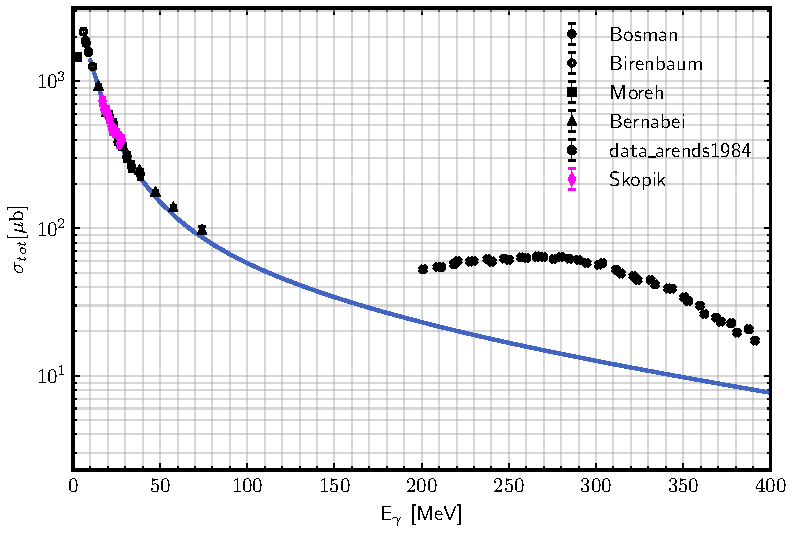
\includegraphics[width=0.75\textwidth]{Figures_python/TOTAL_CROSSSECTION.pdf}
        \end{center}
        \caption{Total cross section as a function of the photon's energy E$_\gamma$.
        Solid blue line presents results obtained with SN+Siegert 
        and dashed pink line - with only SN current.
        The experimental data are from \cite{Bernabei1986} (black filled circles),
        \cite{BOSMAN1979} (empty circles),
        \cite{ARENDS1984} (red squares),
        \cite{Skopik1974} (olive triangles),
        \cite{Moreh1989} (cyan crosses X) and
        \cite{Birenbaum1985} (purple dimonds).
        }
        \label{TOTAL_CROSS}
    \end{figure}
    

    \begin{figure}[h]
        \begin{center}
        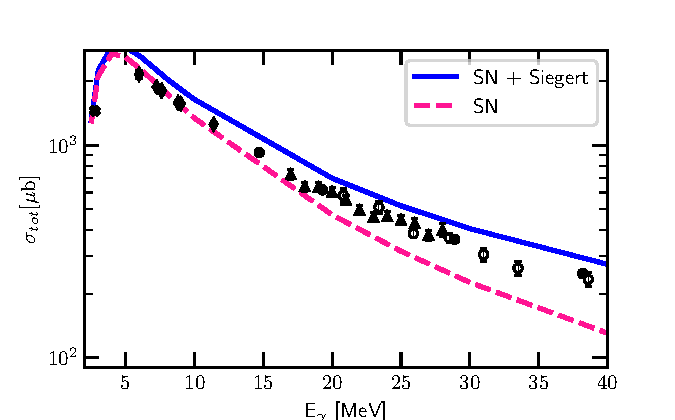
\includegraphics[width=0.75\textwidth]{Figures_python/TOTAL_CROSSSECTION_SMALL_REGION.pdf}
        \end{center}
        \caption{The same as on the Fig.~\ref{TOTAL_CROSS} but for the energy range 2.5 - 80 MeV.
        }
        \label{TOTAL_CROSS_small}
    \end{figure}
        

    \begin{figure}[h]
        \begin{center}
        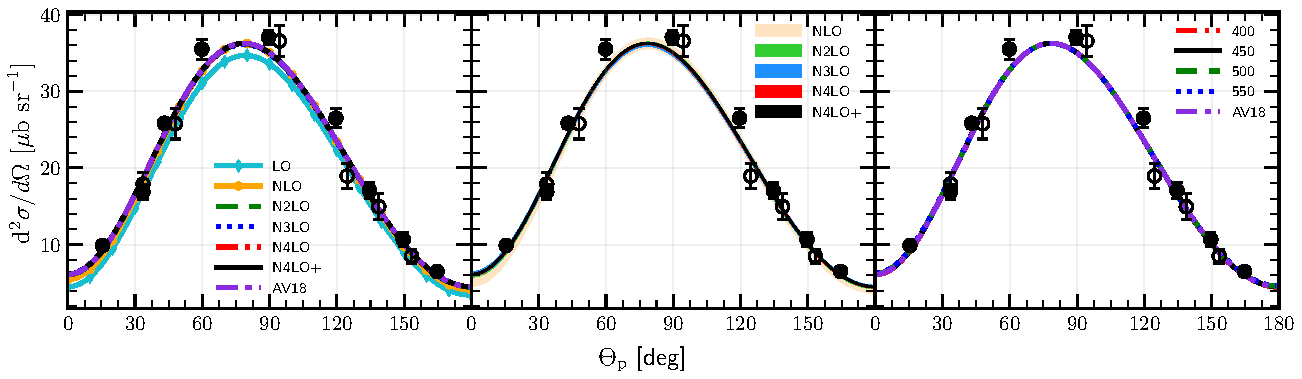
\includegraphics[width=0.95\textwidth]{Figures_python/CROSS2_30mev.pdf}
        \end{center}
        \caption{Differential cross section as a function of the outgoing proton angle in the center of mass frame 
        for the photon's energy 30 MeV. Left figure presents results obtained using potential
        with different chiral orders (from LO to N$^4$LO+) with cutoff parameter $\Lambda=450$~MeV
        whereas right figure presents a cutoff dependency and chiral potential N$^4$LO+ was used in all cases.
        For the sake of comparison, predictions obtained with AV18 potential are on both figures as well.
        Data points (filled and empty circles) are from \cite{Ying_Experiment_Deut}.}
        \label{CROSS_30}
    \end{figure}
        

    \begin{figure}[h]
        \begin{center}
        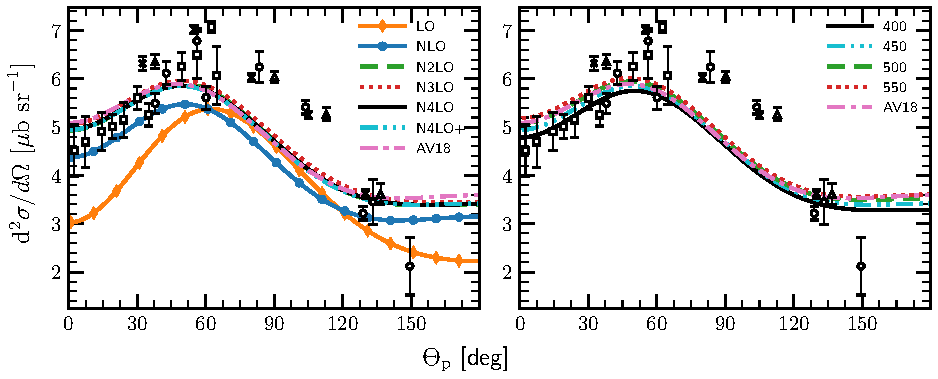
\includegraphics[width=0.95\textwidth]{Figures_python/CROSS2_100mev.pdf}
        \end{center}
        \caption{The same as on the Fig.~\ref{CROSS_30} but for the photon's energy E$_\gamma$=100~MeV.
        All experimental data points (filled and empty circles, squares and triangles) are from \cite{Ying_Experiment_Deut}.}
        \label{CROSS_100}
    \end{figure}

    \begin{figure}[h]
        \begin{center}
        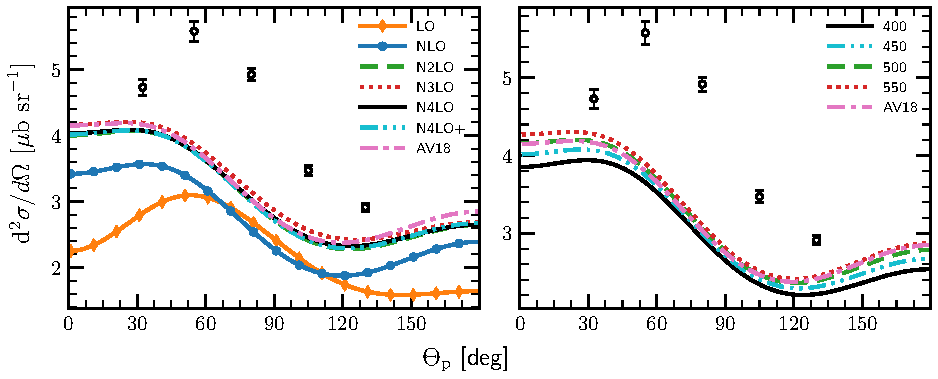
\includegraphics[width=0.95\textwidth]{Figures_python/CROSS2_140mev.pdf}
        \end{center}
        \caption{The same as on the Fig.~\ref{CROSS_30} but for the photon's energy E$_\gamma$=140~MeV.
        The data are from \cite{DeSanctis_Experiment_Deut}.}
        \label{CROSS_140}
    \end{figure}
        



    \begin{figure}[h]
        \begin{center}
        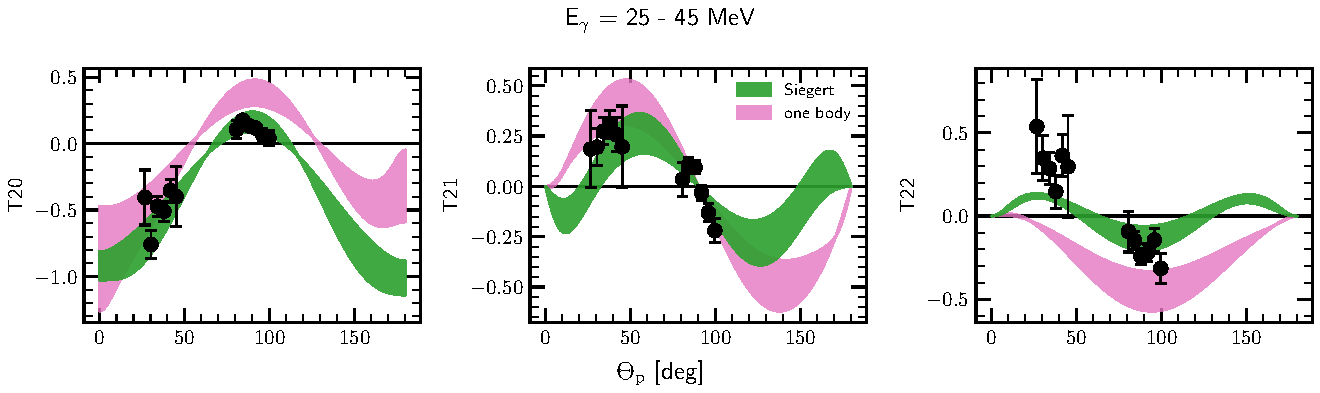
\includegraphics[width=1\textwidth]{Figures_python/Tensor_analyzing_power_angular_E25-45.pdf}
        \end{center}
        \caption{Tensor analyzing powers T$_{20}$, T$_{21}$ and T$_{22}$ as a functions of the
        outgoing proton angle $\theta_p$ (in the center of mass frame).
        Solid blue line is a mean value of my predictions obtained with a
        SMS potential at N$^4$LO+ chiral order and with $\Lambda$~=~450~MeV
        at energy values from 25 to 45 MeV and
        where SN current was used together with Siegert approach. 
        Pink dashed line is similar prediction but with SN only. 
        The corresponding bands show the deviation of predictions in the regarded
        energy region.
        % Filled bands show maximal spread of my predictions obtained with a 
        % SMS potential at N$^4$LO+ chiral order and with $\Lambda$~=~450~MeV
        % for the energy span from 25 to 45 MeV. Blue bands correspond to the
        % case where SN current was used together with Siegert approach and 
        % pink bands - to the SN currentonly. 
        Filled circles are experimental data
        from \cite{rachek2007} for the analogous energy span.}
        \label{tensor_angular_25-45}
    \end{figure}

    \begin{figure}[h]
        \begin{center}
        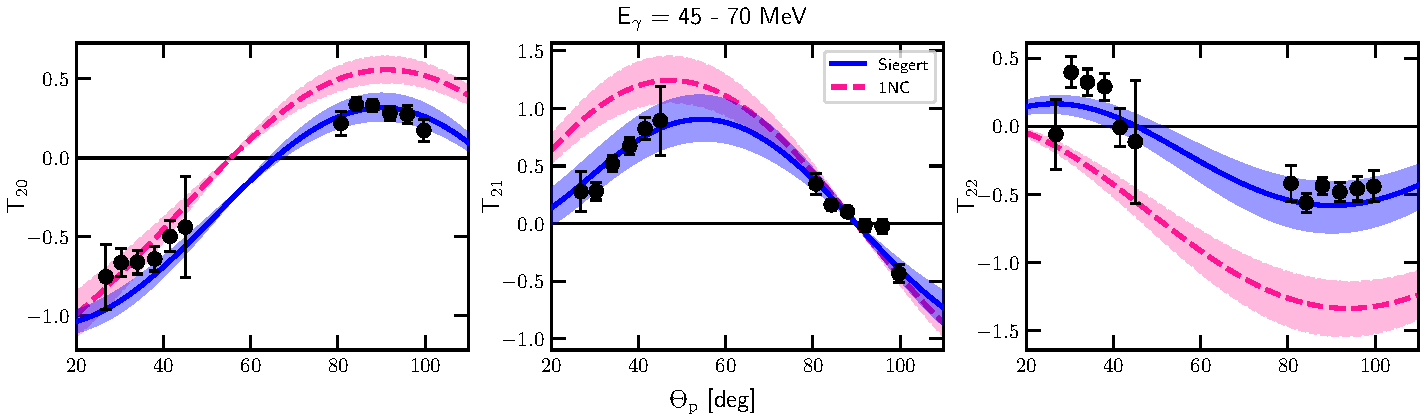
\includegraphics[width=0.95\textwidth]{Figures_python/Tensor_analyzing_power_angular_E45-70.pdf}
        \end{center}
        \caption{The same as on the Fig.~\ref*{tensor_angular_25-45} but for energy bin 45~-~70~MeV}
        \label{tensor_angular_45-70}
    \end{figure}

    \begin{figure}[h]
        \begin{center}
        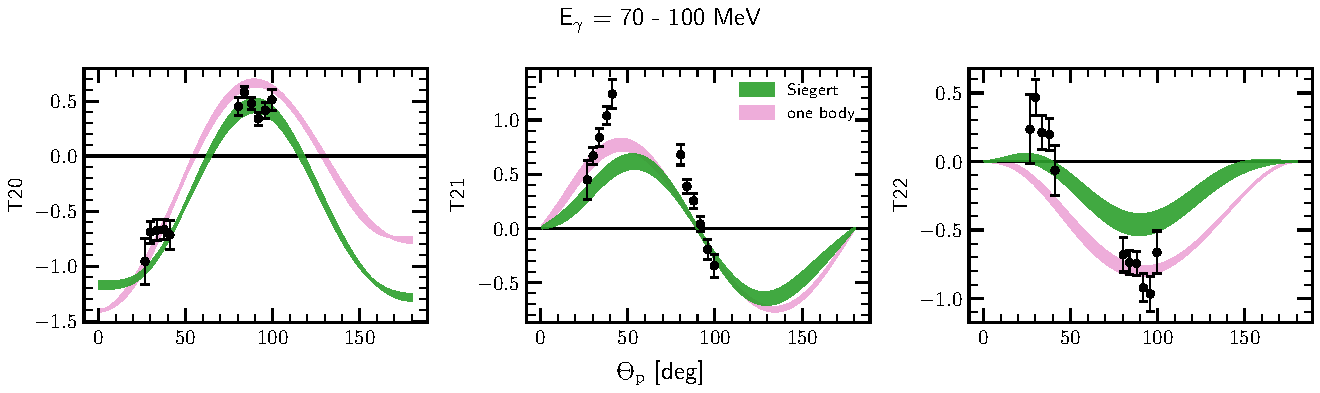
\includegraphics[width=0.95\textwidth]{Figures_python/Tensor_analyzing_power_angular_E70-100.pdf}
        \end{center}
        \caption{The same as on the Fig.~\ref*{tensor_angular_25-45} but for energy bin 70~-~100~MeV}
        \label{tensor_angular_70-100}
    \end{figure}        

    \begin{figure}[h]
        \begin{center}
        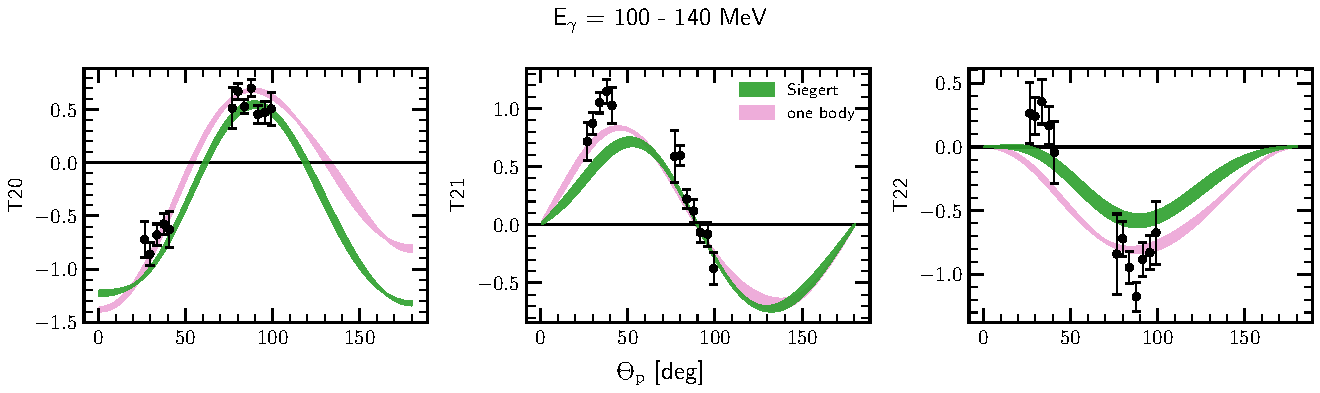
\includegraphics[width=0.95\textwidth]{Figures_python/Tensor_analyzing_power_angular_E100-140.pdf}
        \end{center}
        \caption{The same as on the Fig.~\ref*{tensor_angular_25-45} but for energy bin 100~-~140~MeV}
        \label{tensor_angular_100-140}
    \end{figure}
        
        

    \begin{figure}[h]
        \begin{center}
        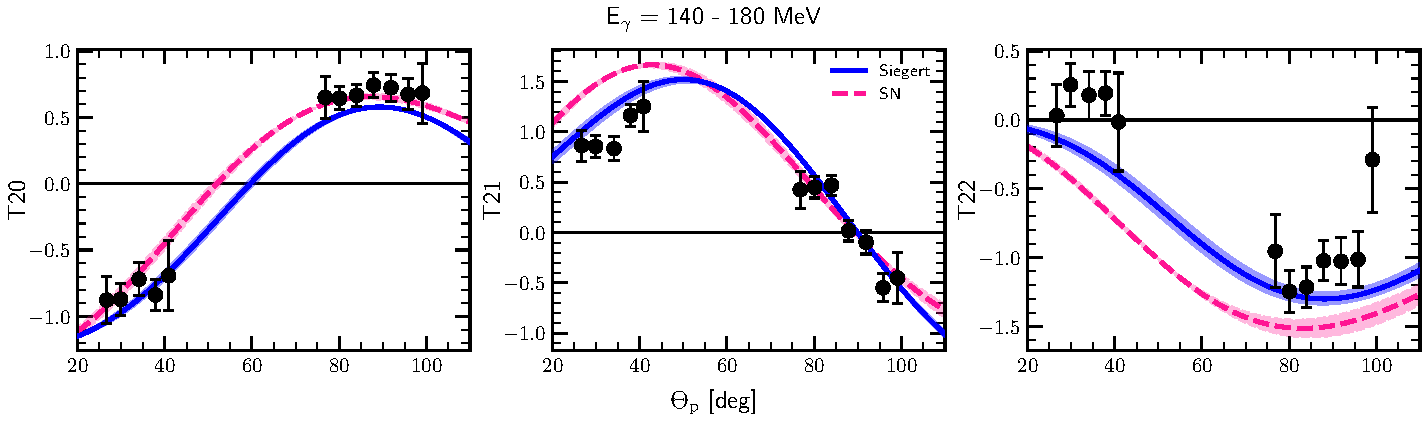
\includegraphics[width=0.95\textwidth]{Figures_python/Tensor_analyzing_power_angular_E140-180.pdf}
        \end{center}
        \caption{The same as on the Fig.~\ref*{tensor_angular_25-45} but for energy bin 140~-~180~MeV}
        \label{tensor_angular_140-180}
    \end{figure}
        

    \begin{figure}[h]
        \begin{center}
        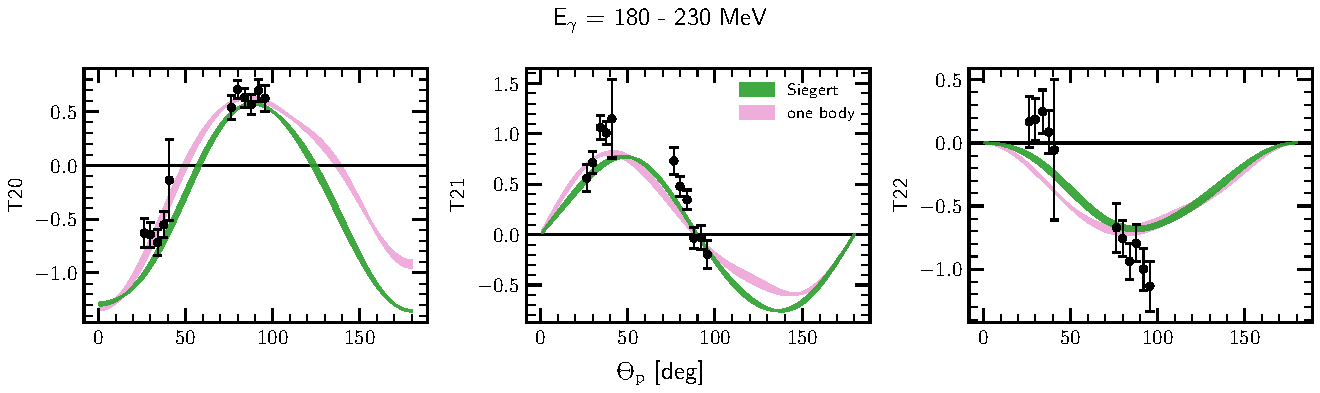
\includegraphics[width=0.95\textwidth]{Figures_python/Tensor_analyzing_power_angular_E180-230.pdf}
        \end{center}
        \caption{The same as on the Fig.~\ref*{tensor_angular_25-45} but for energy bin 180~-~230~MeV}
        \label{tensor_angular_180-230}
    \end{figure}

    \begin{figure}[h]
        \begin{center}
        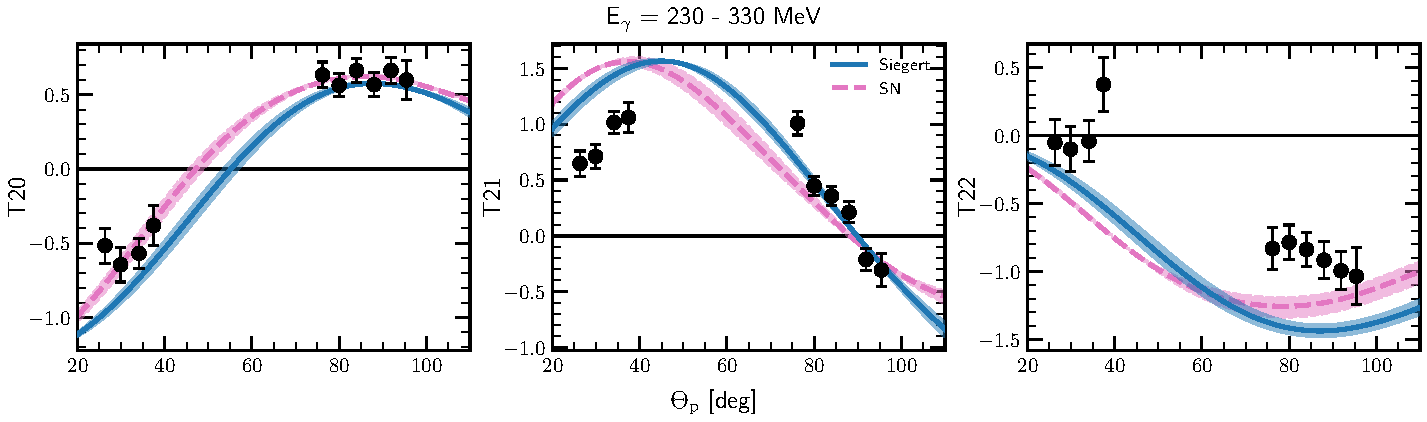
\includegraphics[width=0.95\textwidth]{Figures_python/Tensor_analyzing_power_angular_E230-330.pdf}
        \end{center}
        \caption{The same as on the Fig.~\ref*{tensor_angular_25-45} but for energy bin 230~-~330~MeV}
        \label{tensor_angular_230-330}
    \end{figure}
        


    \begin{figure}[h]
        \begin{center}
        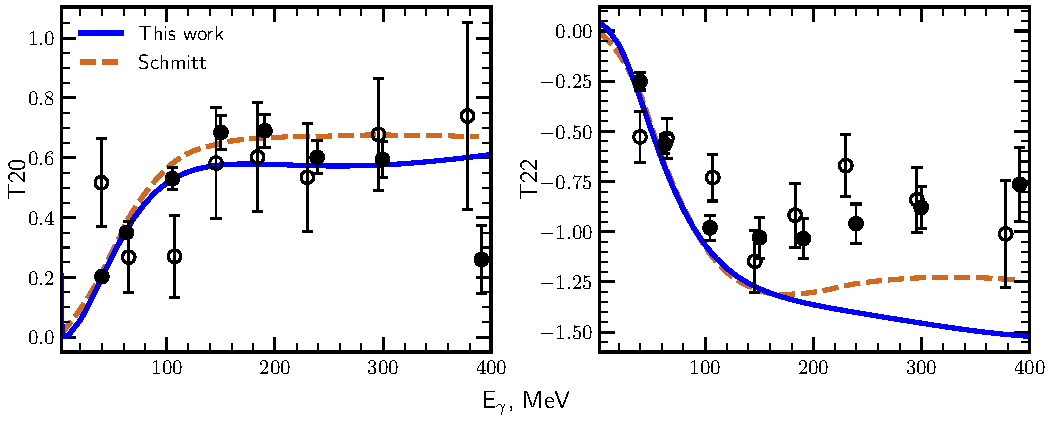
\includegraphics[width=0.75\textwidth]{Figures_python/T20_T22_vs_en.pdf}
        \end{center}
        \caption{Tensor analyzing powers T$_{20}$ and T$_{22}$ as a functions of the photon energy E$_\gamma$
        with fixed outgoing proton angle $\theta_p = 88^{\circ}$ (in the center of mass frame).
        My predictions (blue solid line) are obtained with SMS potential at chiral order N$^4$LO+
        and with cutoff parameter $\Lambda$~=~450~MeV.
        Dashed purple line presents calculations from \cite{Schmitt1989}.
        Experimental data is taken from \cite{rachek2007} (filled circles)
        and \cite{mishev1993} (empty circles).}
        \label{T20_vs_en}
    \end{figure}

    \begin{figure}[h]
        \begin{center}
        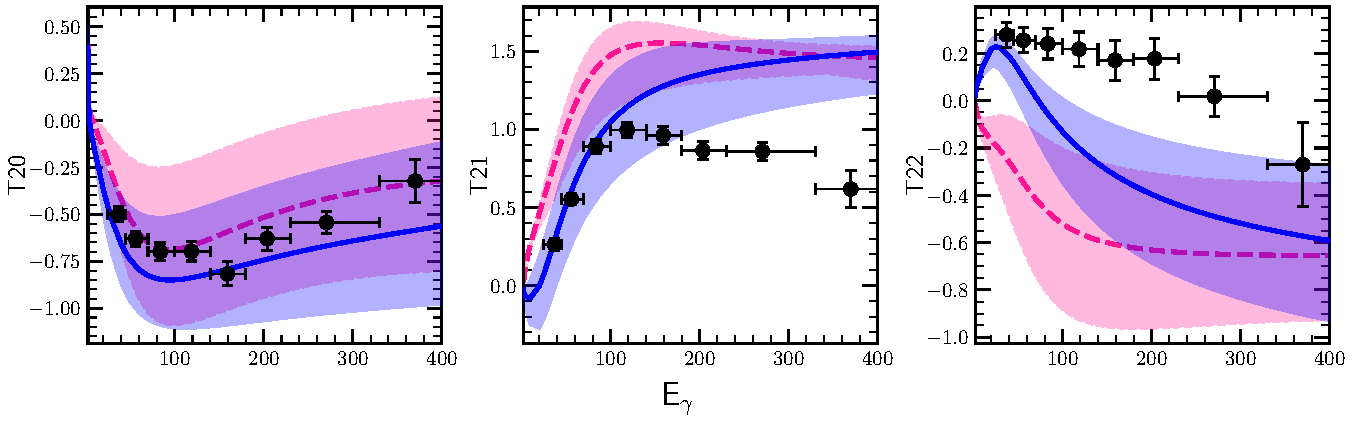
\includegraphics[width=0.95\textwidth]{Figures_python/TensorPower_Th24-48.pdf}
        \end{center}
        \caption{Tensor analyzing powers T$_{20}$, T$_{21}$ and T$_{22}$ as a functions of the
        photon's energy within the outgoing proton's angle range $24^{\circ} - 48^{\circ}$
        (in the center of mass frame).
        Solid blue line is a mean value of my predictions obtained with
        SMS potential at N$^4$LO+ chiral order and with $\Lambda$~=~450~MeV
        at energy values from 25 to 45 MeV within
        a given angles range and
        where SN current was used together with Siegert approach. 
        Pink dashed line is similar prediction but with SN only. 
        The corresponding bands show the deviation of predictions in the regarded
        energy region.
        Filled circles are experimental data
        from \cite{rachek2007} for the analogous energy span.}
        \label{tensor_energy_24-48}
    \end{figure}

    \begin{figure}[h]
        \begin{center}
        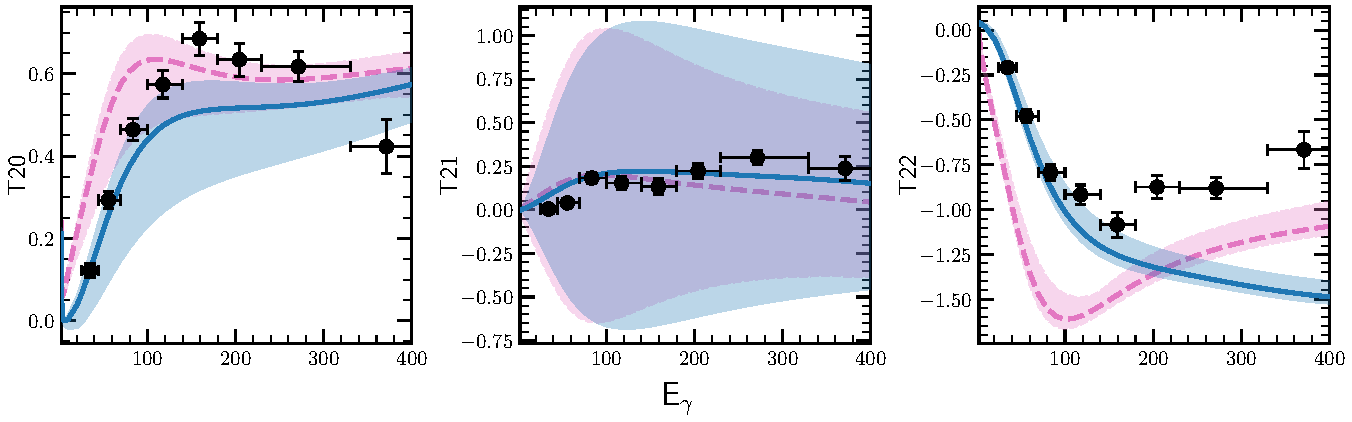
\includegraphics[width=0.95\textwidth]{Figures_python/TensorPower_Th70-102.pdf}
        \end{center}
        \caption{The same as on the Fig.~\ref*{tensor_energy_24-48} but
        for the angles' range $70^{\circ} - 102^{\circ}$.}
        \label{tensor_energy_70-102}
    \end{figure}
        
    % I will try to figure out why we can see such a wide band of predictions
    % for $T_{20}$ in the Fig.~\ref*{tensor_energy_24-48} and
    % for $T_{21}$  in the Fig.~\ref*{tensor_energy_70-102}.
    % Let's stick to the particular energy value E$_\gamma = 120$~MeV.
    % The spread of predictions is high in the both cases for such energy value.
    % The corresponding angular distribution of these observables
    % one can find on the  Fig.~\ref*{tensor_angular_100-140}
    % (of course there is some energy range on the Figure, but let's assume that 
    % energy dependance is not so strong around 120~MeV and for $T_{20}$
    % it is confirmed by the Fig.~\ref*{T20_vs_en}).
    % In the first case we have a prediction for angles' range $24^{\circ} - 48^{\circ}$
    % and we can see that $T_{20}$ in this region has 